As with any high-dimensional optimization problem, the fitter must be vigilant
against the overfitting of data. In practice, this requires:

parsimony with the number of parameters used in the model

common-sense checking "under the hood" of the optimization to verify that
parameter values make sense given the assumptions that undergird the model

understanding of what the value function is (that is, the function being
minimized/maximized) and whether it needs to be changed

cross-correlation between parameters to understand the relationship between
parameters and the effect that each has on predictions made using the model

TCS affected by HF parameters, spin orbit, imaginary above
RCS affected by imaginary above, HF parameters
ECS affected by HF parameters, spin orbit, imaginary above
APower affected by HF parameters, spin orbit,  imaginary above
Charge Density affected by HF parameters, imaginary below
Levels affected by HF parameters, spin orbit,
Spectral functions affected by HF parameters, imaginary below
RMSRadii affected by HF parameters, imaginary below

Physical intuition about scattering data:
- the low-angle ECS/APower data are sensitive to the imaginary strength above
the Fermi surface. The high-angle ECS/APower data are sensitive to the imaginary
strength below the Fermi surface, with the highest angles of elastic scattering
probing the imaginary strength deepest in the core (see high-energy, high-angle
data in Pb)
- the NM correction to the imaginary volume strength is required in all cases to
have the very high/very low energy imaginary strength have the correct trend
(linearly increasing above 100 MeV above, decreasing to 0 below 100 MeV below).
Seen in spectral functions and total cross section data at high energies, where
the pion production channel enters the picture as it goes from virtual->real
- the general trend of the elastic scattering data (not wiggles, but averaged
over wiggles) depends on the imaginary strength at the given energy. If the
minima in the elastic cross sections are too sharp/deep, the imaginary strength
is too large at that energy
- the spin-orbit strength has dramatic effects on the total cross section at low
energies ($<$20 MeV)
- above the Fermi surface, the imaginary strength is dominated by surface from
0-50 MeV and by volume from 50 MeV up. Below the Fermi surface, the surface
imaginary strength is dependent on A; for low A, where the level density is very
low below the Fermi surface and there's almost no contribution from high LJ
levels, there is virtually no surface imaginary strength below (cf. with charge
density distribution tail, at the surface of the nucleus). As A increases, 
imaginary surface strength below increases gradually but never reaches the
imaginary surface strength above. A consequence of the asymmetry of the
operators that contribute: below 0 MeV, the removal operator LJs
must recouple to the ground state, so high LJ operators have virtually no
contribution; above 0 MeV, addition operators can have arbitrary LJs because
free scattering is possible, adding significantly to the collective strength and
thus is imaginary strength peaked at the surface in the 20-30 MeV range (giant
dipole resonance, for example, surface phonons).

\subsection{Fitting procedure}
The powell method, outlined in Numerical Recipes in C \cite{NumericalRecipes},
was used to minimize the RMS difference between experimental data points and the
values calculated by the DOM. A weighting scheme was assigned to the data points
according to their importance, guiding the fit to reproduce the most essential
data points. From fit to fit, the weighting scheme was adjusted as necessary to
escape local minima in the multidimensional fit.

The radial grid, energy grid, size of the lagrange basis, partial wave angular momentum cutoff, and
various integration cutoffs used in calculating the potential and
observable quantities were varied to ensure that output was not distorted by numerical errors. 

\subsection{Treatment of open neutron shells}

\section{Results for \oSix}
As the lightest system yet analyzed in the DOM framework, \oSix is a useful test case
for the validity of the DOM in light systems and useful benchmark for $\chi$-EFT, shell model, ab
initio approaches, and other theoretical treatments. In addition, a wealth of scattering and
bound-state information have been collected on this nucleus that expose the strengths and
weaknesses of the DOM potential forms.

Detailed results of the experimental data used to constrain the \oSix potential and the resulting
fit are available in Fig \ref{insert figures} in Appendix A. Good agreement with all experimental
data was achieved, excepting the following regimes:

- neutron total cross section at <10 MeV
- proton differential elastic cross sections and analyzing powers above 150 MeV at backward angles

For a system as light as \oSix, the density of states at low energies (i.e., below the neutron
separation energy) is sufficiently low that a smoothly-varying potential will be a poor
approximation of the resonance structure that dictates the strength of inelastic scattering. Hence,
our fit of the neutron total cross section in \oSix fails to reproduce the resonance structures and
instead generates an average behavior over these resonances.

\section{Results for \oEight}
Of the nuclides we chose for a DOM treatment, \oEight was the most difficult due to the paucity of
available experimental data, the lightness of the system, and the neutron open shell. To constrain the negative-energy domain
of the potential, the only available experimental data were the neutron and proton separation
energies and the RMS charge radius of \oEight and \neEight. Accordingly, the uncertainty in our extracted structural quantities is
larger than in any other system we studied.

Because no \oEight charge density distribution was available, we generated an approximate charge density
distribution for \oEight by linearly scaling
the radii and densities of the \oSix charge density distribution to reproduce the \oEight RMS charge
radius and maintain a total charge of 8. The reported RMS charge radii of \oSix and \oEight differ by only
0.01 fm (<0.5\%), so the approximate \oEight charge density distribution we generated is barely
distinguishable from the \oSix distribution. This same scaling procedure was also employed to
generate a charge density distribution for \snTwelve, using the
experimentally-derived \snFour charge density distribution. To initiate the fit, the \oSix best-fit parameter values
were assigned to the \oEight parameter file and calculated observables were generated to compare
with \oEight data. Unsurprisingly, the \oSix parameter values were moderately successful at reproducing
the \oEight scattering data without further adjustment, though almost no neutron scattering data is
available besides our newly-measured \tot. Using the \oSix parameters, the \oEight valence SP levels were underbound
by several MeV and the recovered particle number was too low, clearly a result of the insufficient
depth of the \oSix HF term compared to that required for additional binding in \oEight. Thus, before
loosening any other parameters, the HF depth and HF depth asymmetry terms were allowed to vary,
reducing the chi-square contribution from the charge density, particle number, and energy level
sectors. Once a chi-square minimum had been reached with these two parameters, all other symmetric parameters
were allowed to vary.

\section{Results for \caForty}
OMs have been applied to \caForty more than almost any other nucleus. A great deal of high-quality
elastic and inelastic nucleon scattering data, quasi-free scattering data, and elastic electron
scattering data are available to constrain fit parameters both above and below the Fermi surface. In
addition, \caForty is an essential benchmark on the chart of nuclides, within reach for both no-core
shell model (NCSM) and density functional theory (DFT) calculations, and has also been the subject
of earlier DOM treatments.

The structural information of \caForty we extract from the fit
presented here shows significant occupation depletion compared to the mean-field expectation,
unsurprising considering the well-known results of (e,e'p) experiments and correlated nucleon knockout
experiments conducted at Jefferson Lab. In Fig. \ref{s1Depletion}, is clear that without $\approx$30\%
depletion of the proton 1\sOne\ shell, it is impossible to recover the charge density at the core of
\caForty, a characteristic failure of mean-field models that cannot account for depletion. Thanks to 

\section{Results for \caEight}

\section{Results for \niEight}

\section{Results for \niFour}

\section{Results for \snTwelve}

\section{Results for \snFour}

\section{Results for \pbEight}
The size of the neutron skin of \pbEight has been identified by numerous studies as highly
correlated with the density-dependence of the symmetry energy, $L$, a critical input for the neutron
star equation-of-state. By employing parity-violating electron scattering to probe the
weak charge distribution in \pbEight, the PREX experiment at Jefferson Laboratory extracted a
\pbEight neutron skin value of 0.33$\pm$0.17 fm. A followup experiment with improved statistics, PREX II,
is slated to run later in 2019, and is expected to constrain the \pbEight neutron skin thickness to
within 0.06 fm. Given the wide range of \pbEight neutron skin thicknesses predicted by relativistic
and non-relativistic mean-field models, an accurate calculation of this quantity is an excellent
test for the validity of the DOM treatment.

\begin{figure}
\begin{center}
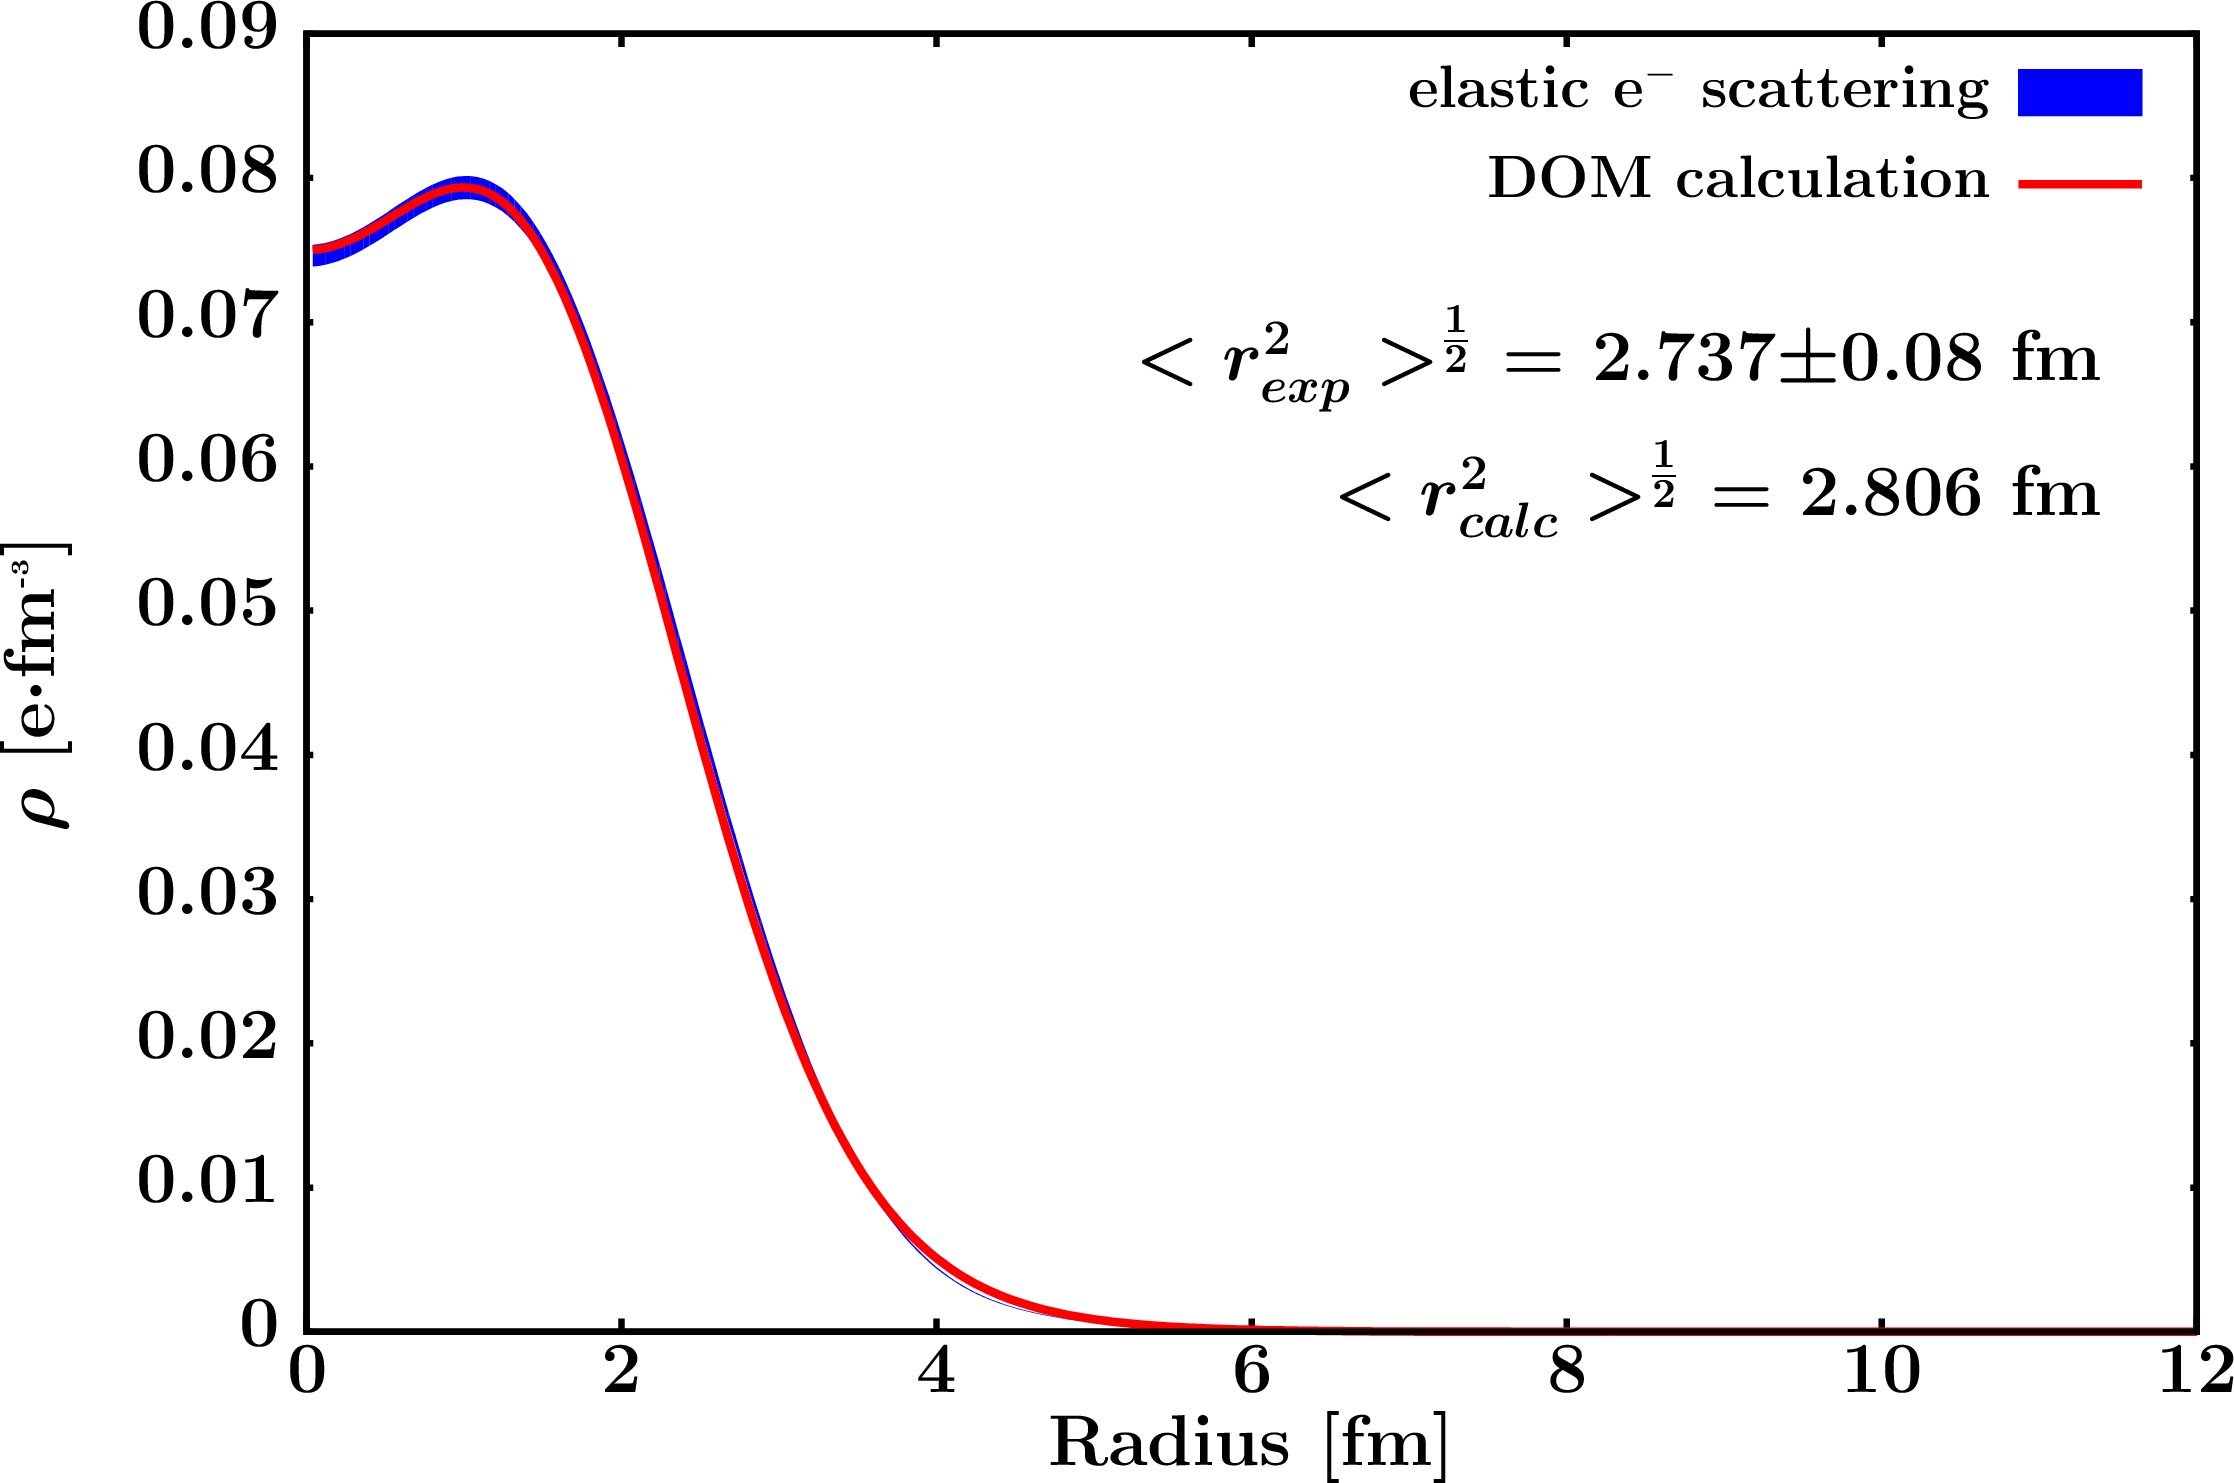
\includegraphics[width = 0.9\textwidth]{figures/o16_chargeDensity.png}
\caption{DOM fit of $^{16}O$ charge density}
\label{o16ChargeDensity}
\end{center}
\end{figure}

\begin{figure}
\begin{center}
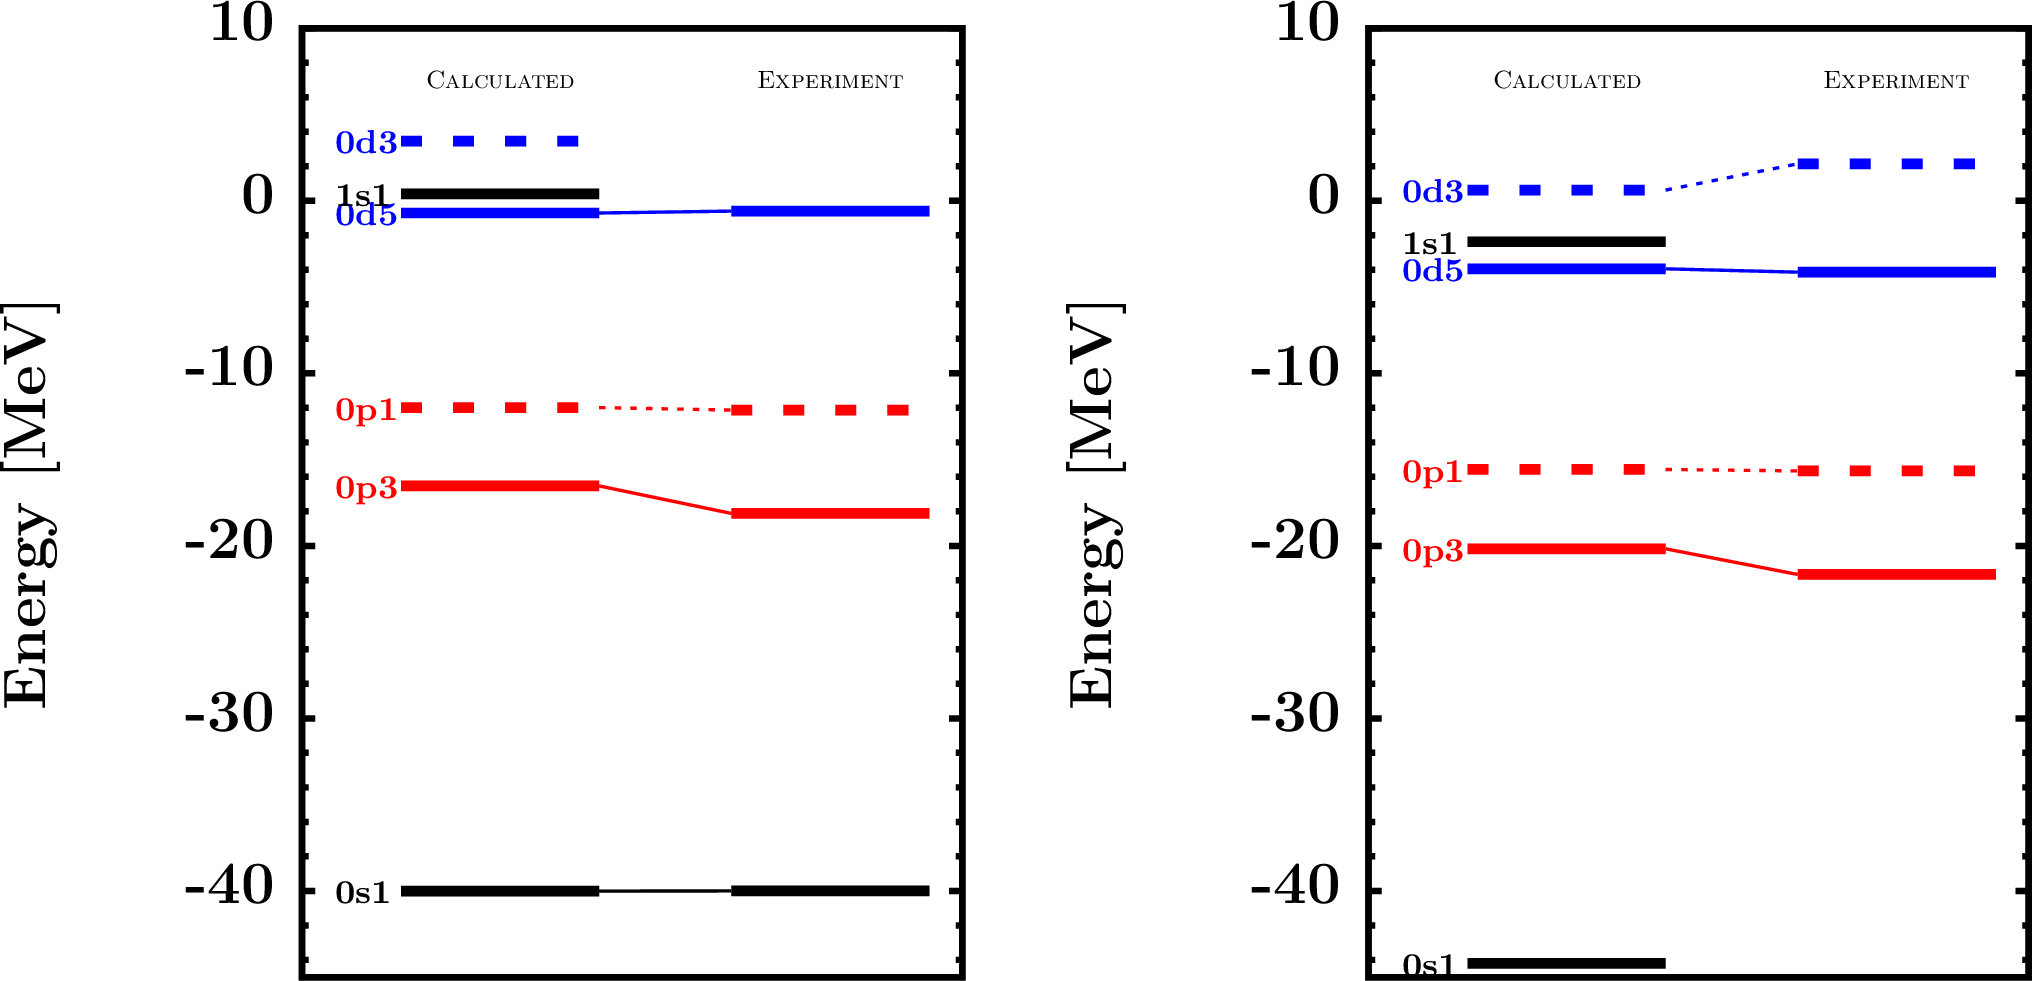
\includegraphics[width = 0.9\textwidth]{figures/o16_SPLevels.png}
\caption{DOM fit of $^{16}O$ single-particle levels}
\label{o16SPLevels}
\end{center}
\end{figure}

\begin{figure}
\begin{center}
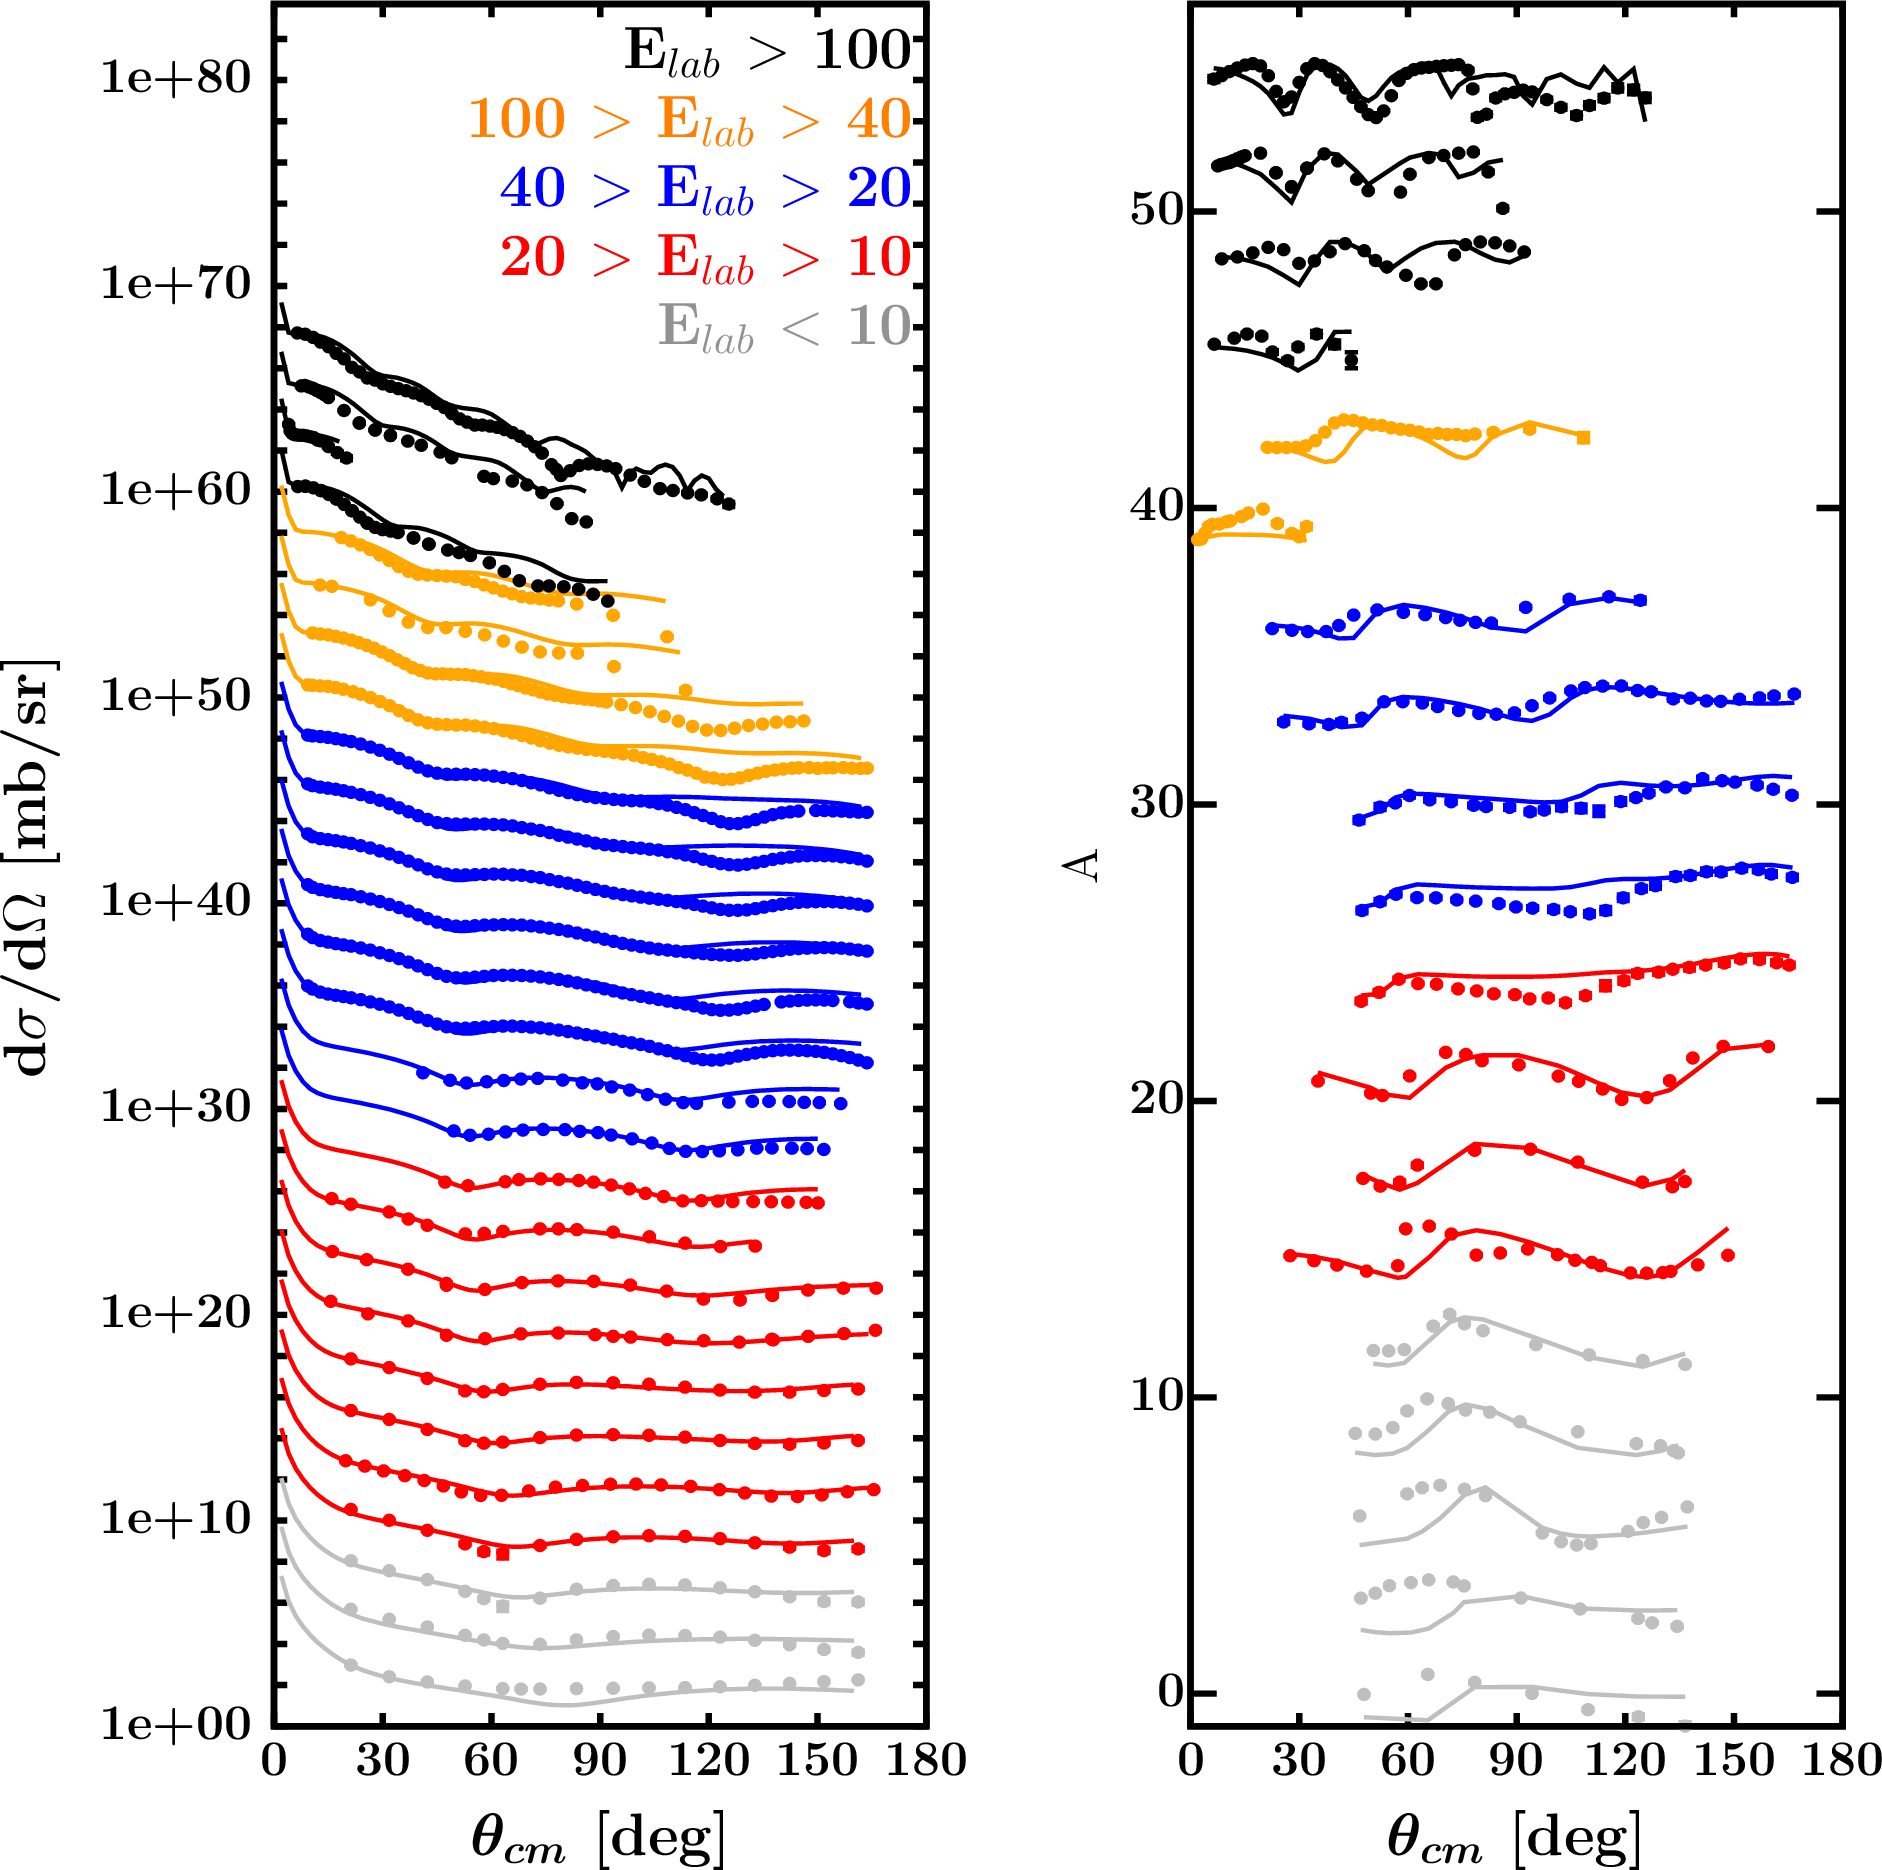
\includegraphics[width = 0.9\textwidth]{figures/o16_protonElastic.png}
\caption{DOM fit of $^{16}O$ proton elastic scattering data}
\label{o16ProtonElastic}
\end{center}
\end{figure}

\begin{figure}
\begin{center}
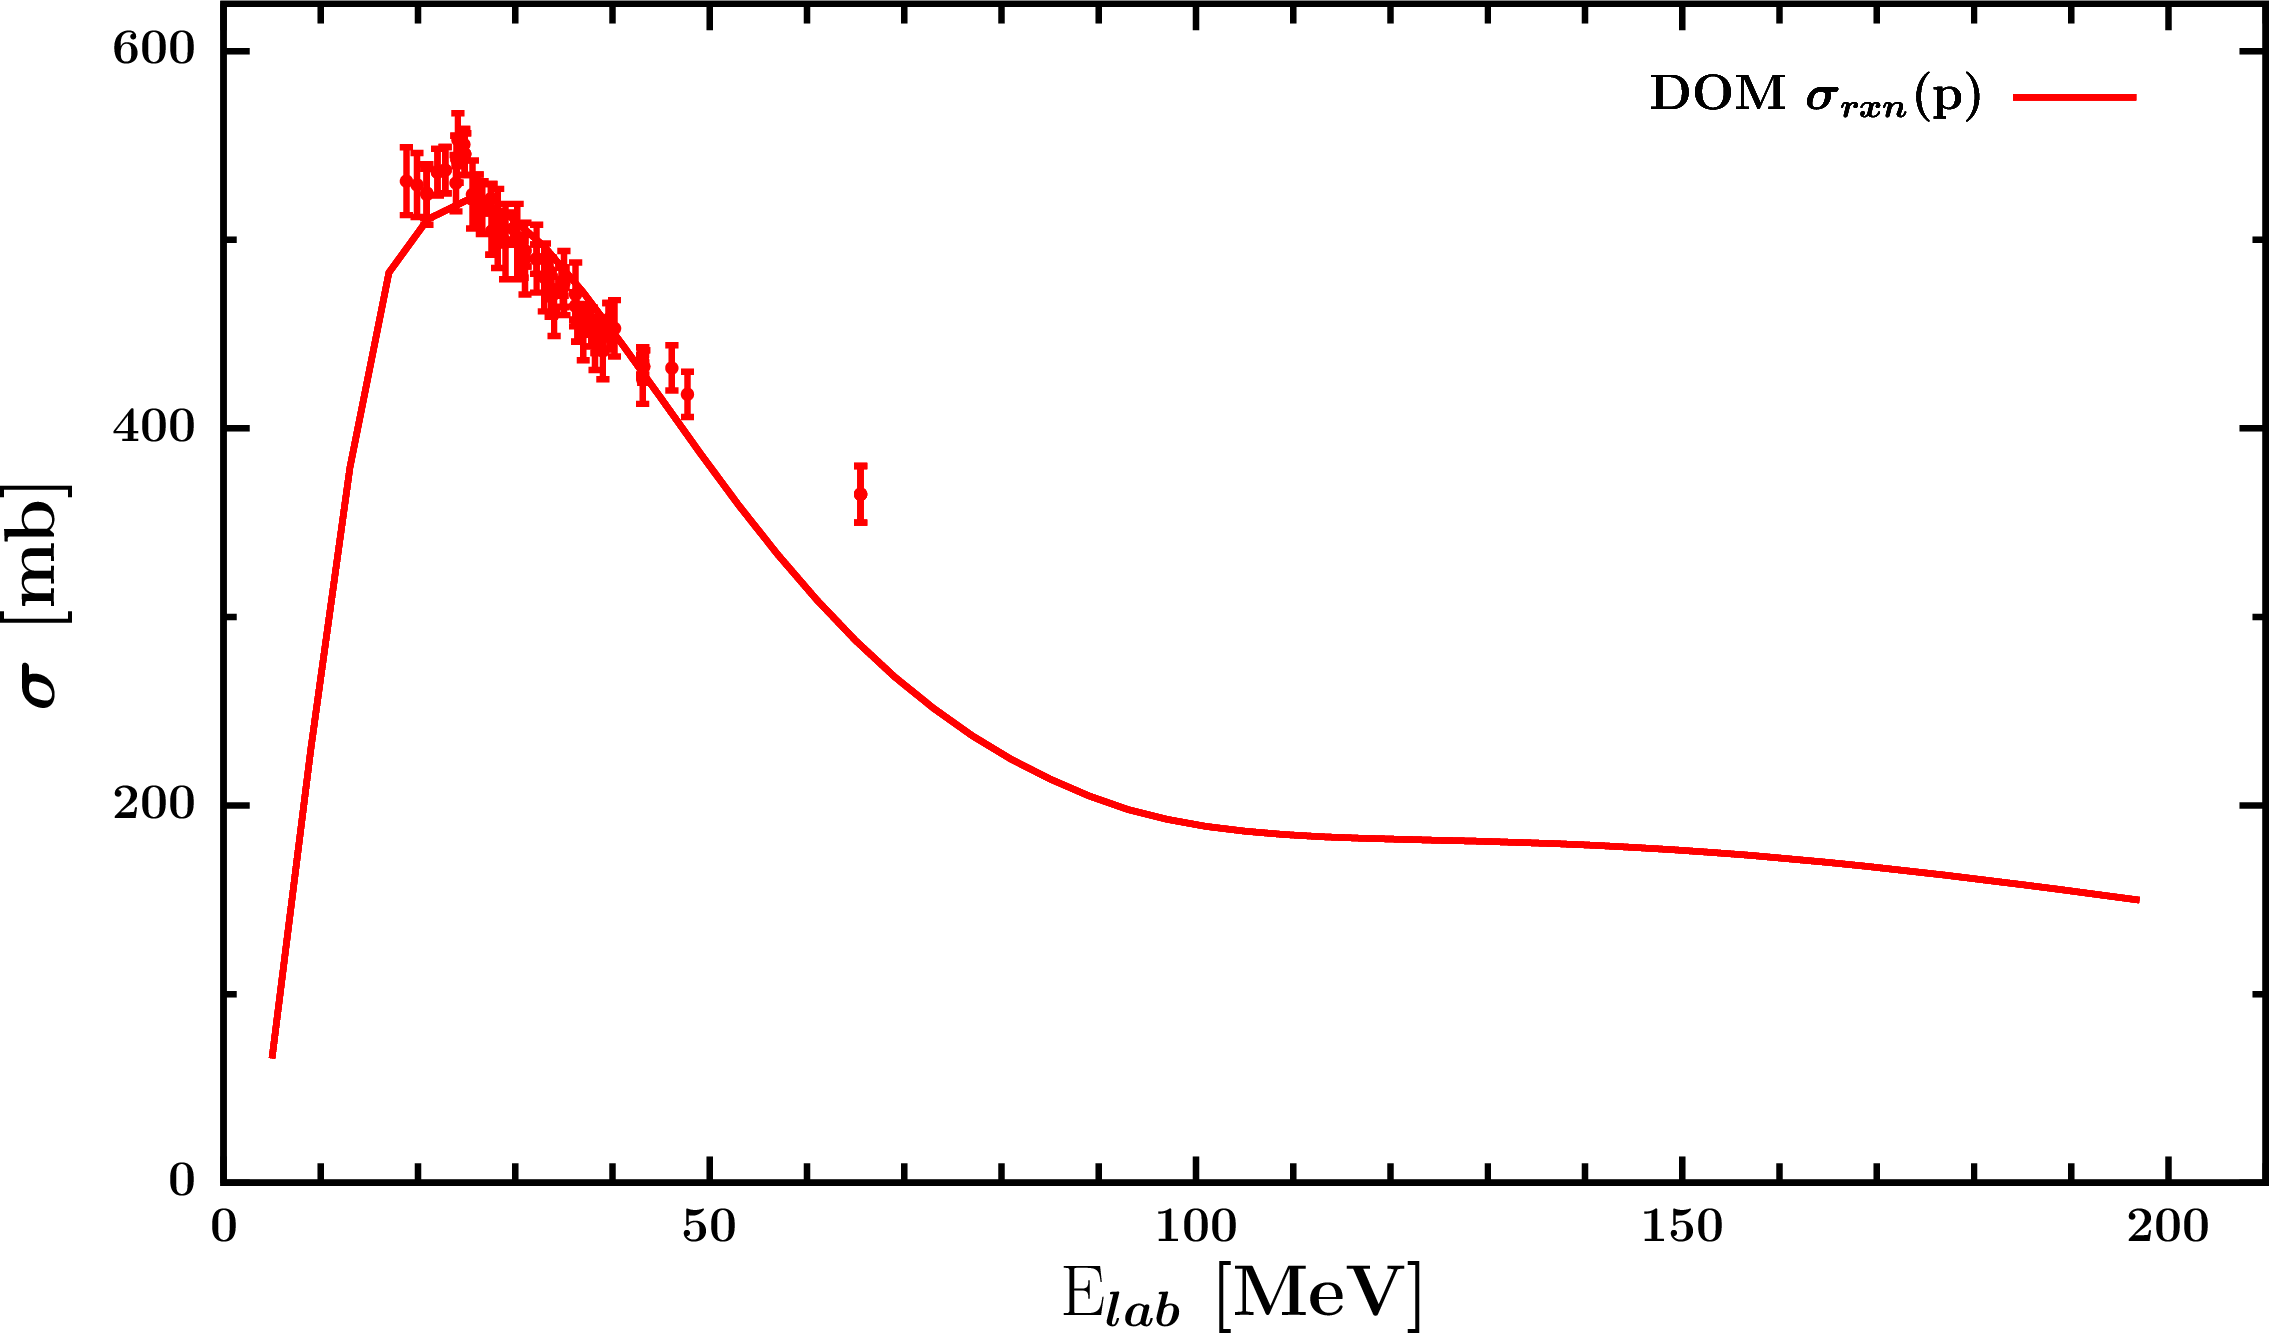
\includegraphics[width = 0.9\textwidth]{figures/o16_protonInelastic.png}
\caption{DOM fit of $^{16}O$ proton inelastic scattering data}
\label{o16ProtonInelastic}
\end{center}
\end{figure}

\begin{figure}
\begin{center}
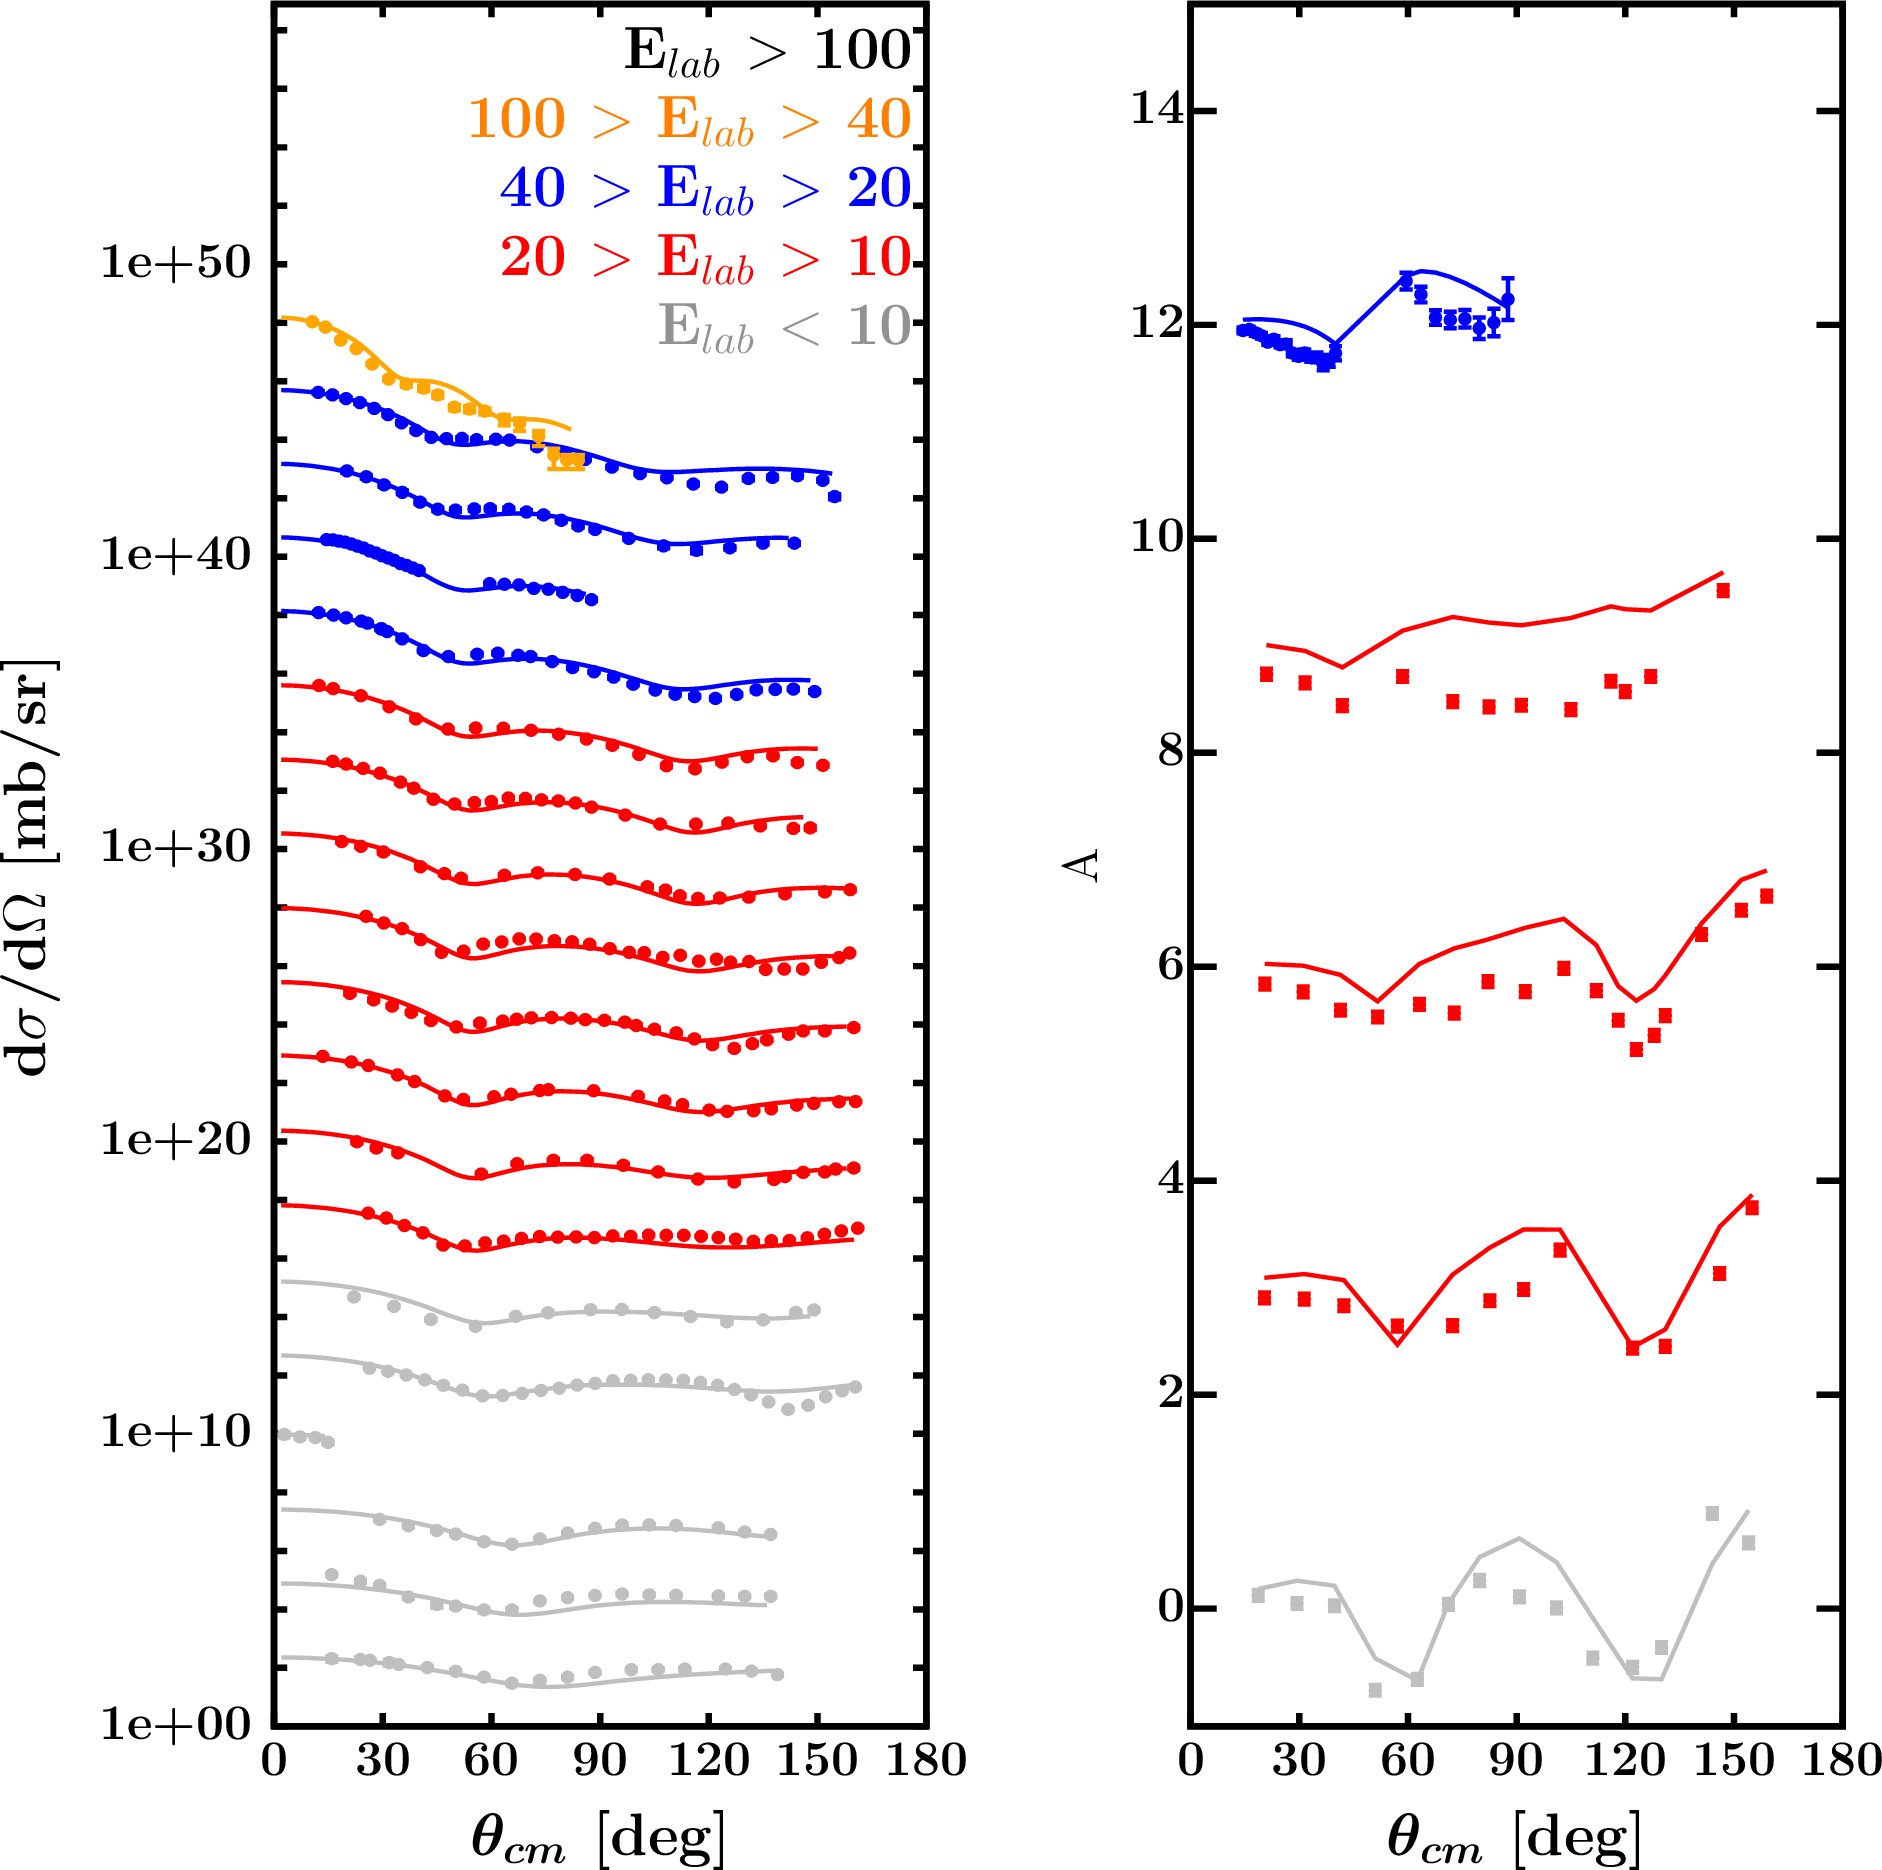
\includegraphics[width = 0.9\textwidth]{figures/o16_neutronElastic.png}
\caption{DOM fit of $^{16}O$ neutron elastic scattering data}
\label{o16NeutronElastic}
\end{center}
\end{figure}

\begin{figure}
\begin{center}
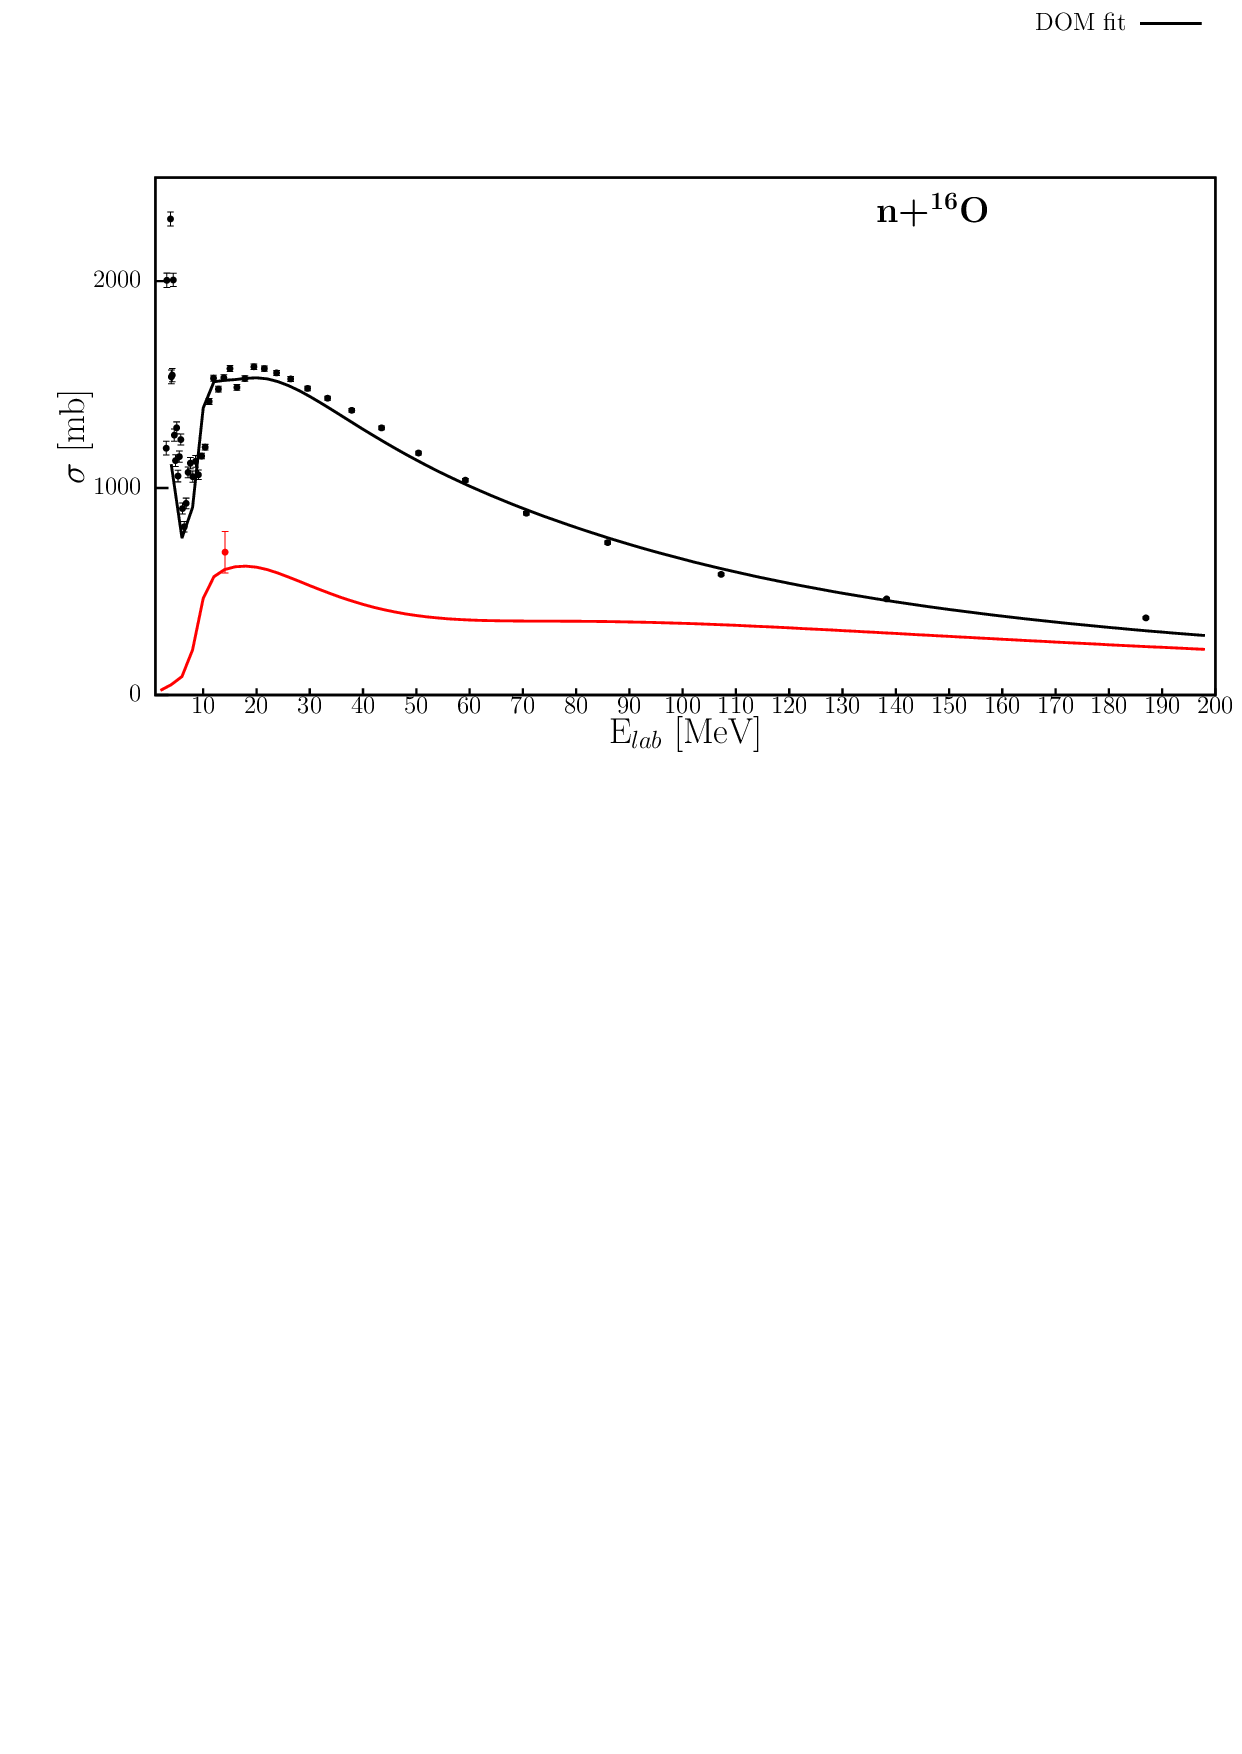
\includegraphics[width = 0.9\textwidth]{figures/o16_neutronInelastic.png}
\caption{DOM fit of $^{16}O$ neutron inelastic scattering data}
\label{o16NeutronInelastic}
\end{center}
\end{figure}

\begin{figure}
\begin{center}
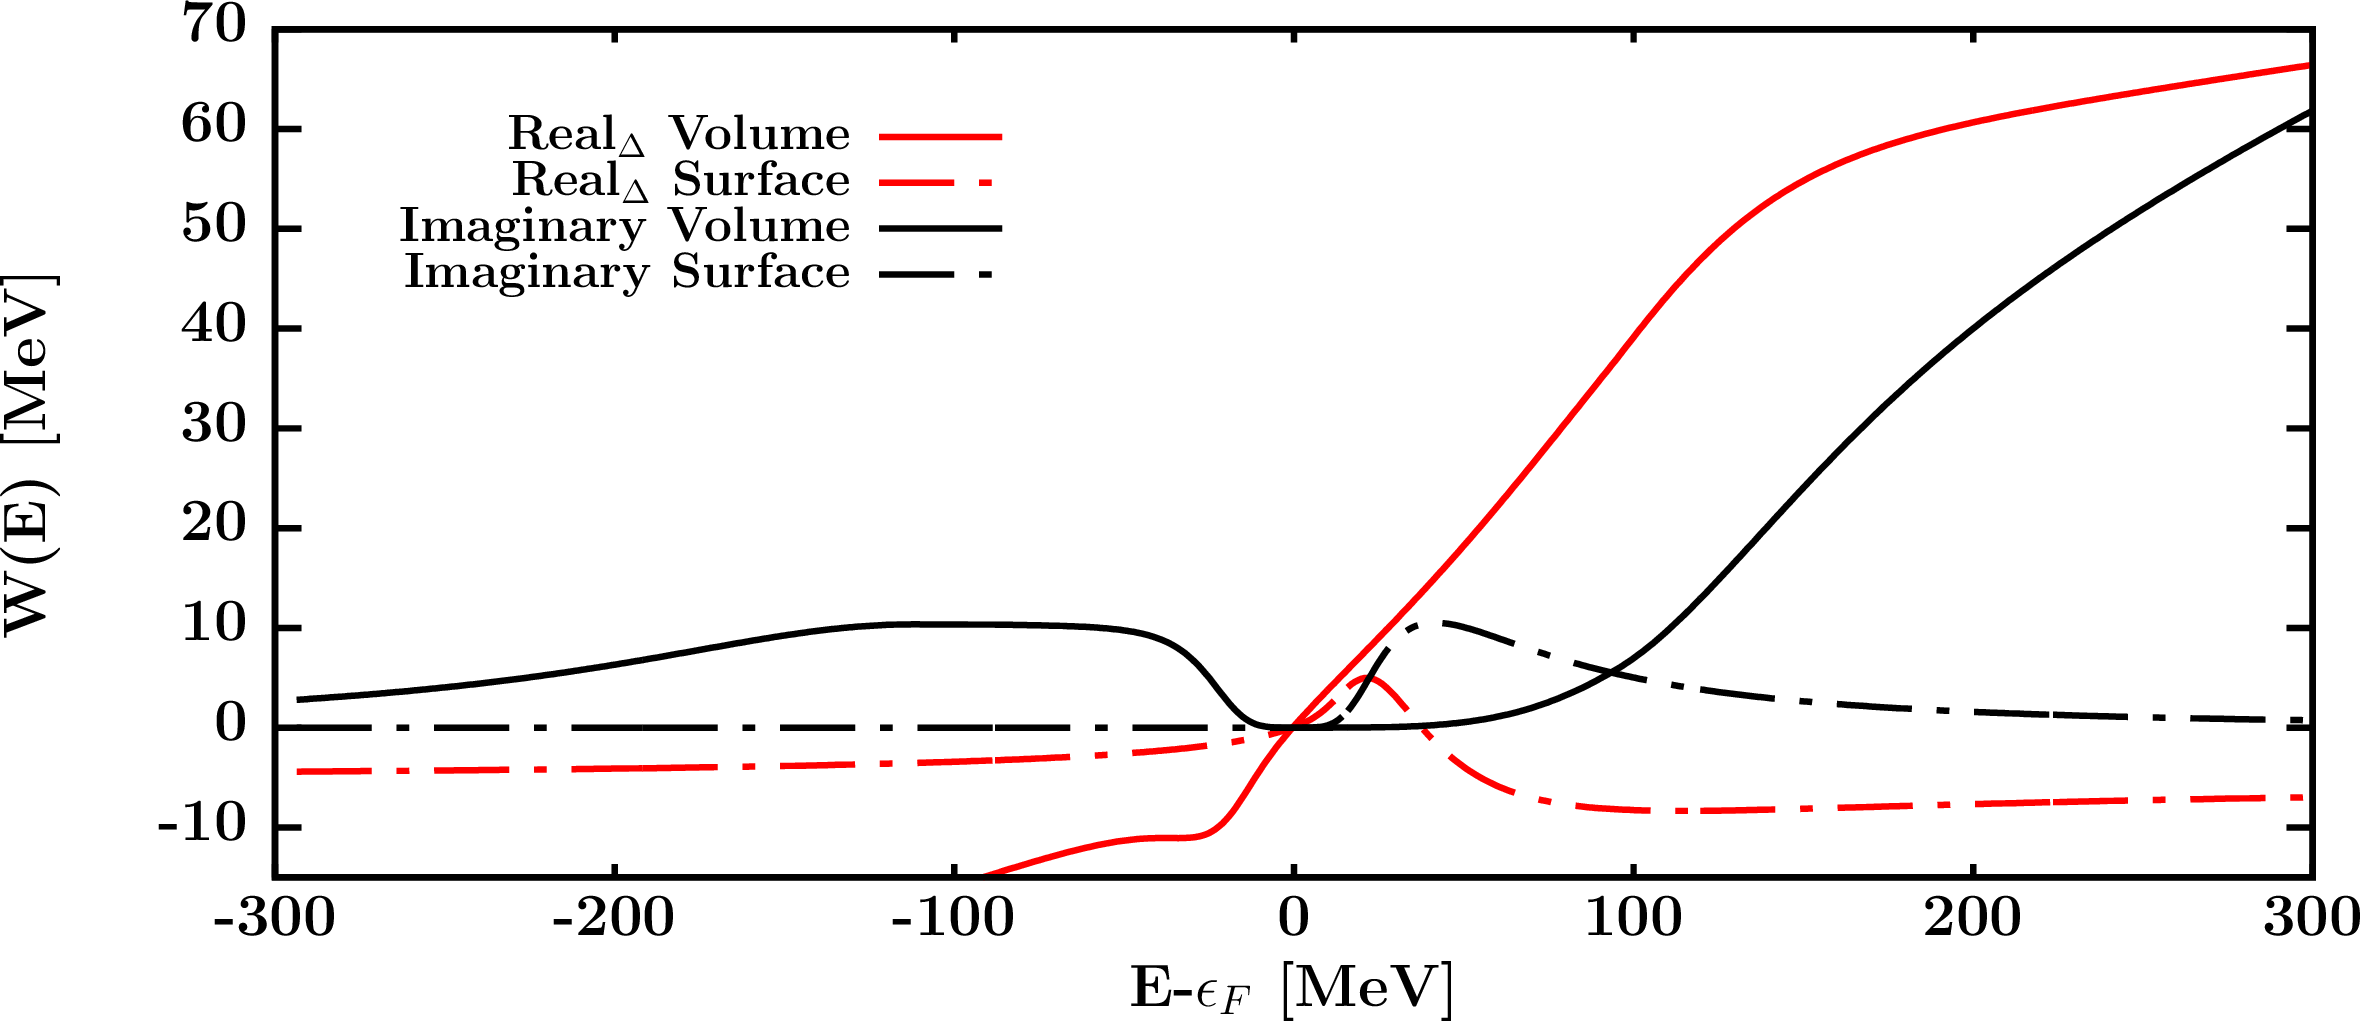
\includegraphics[width = 0.9\textwidth]{figures/o16_protonPotentials.png}
\caption{Visualization of DOM optical potential components for protons on
$^{16}O$}
\label{o16ProtonPotentials}
\end{center}
\end{figure}

\begin{figure}
\begin{center}
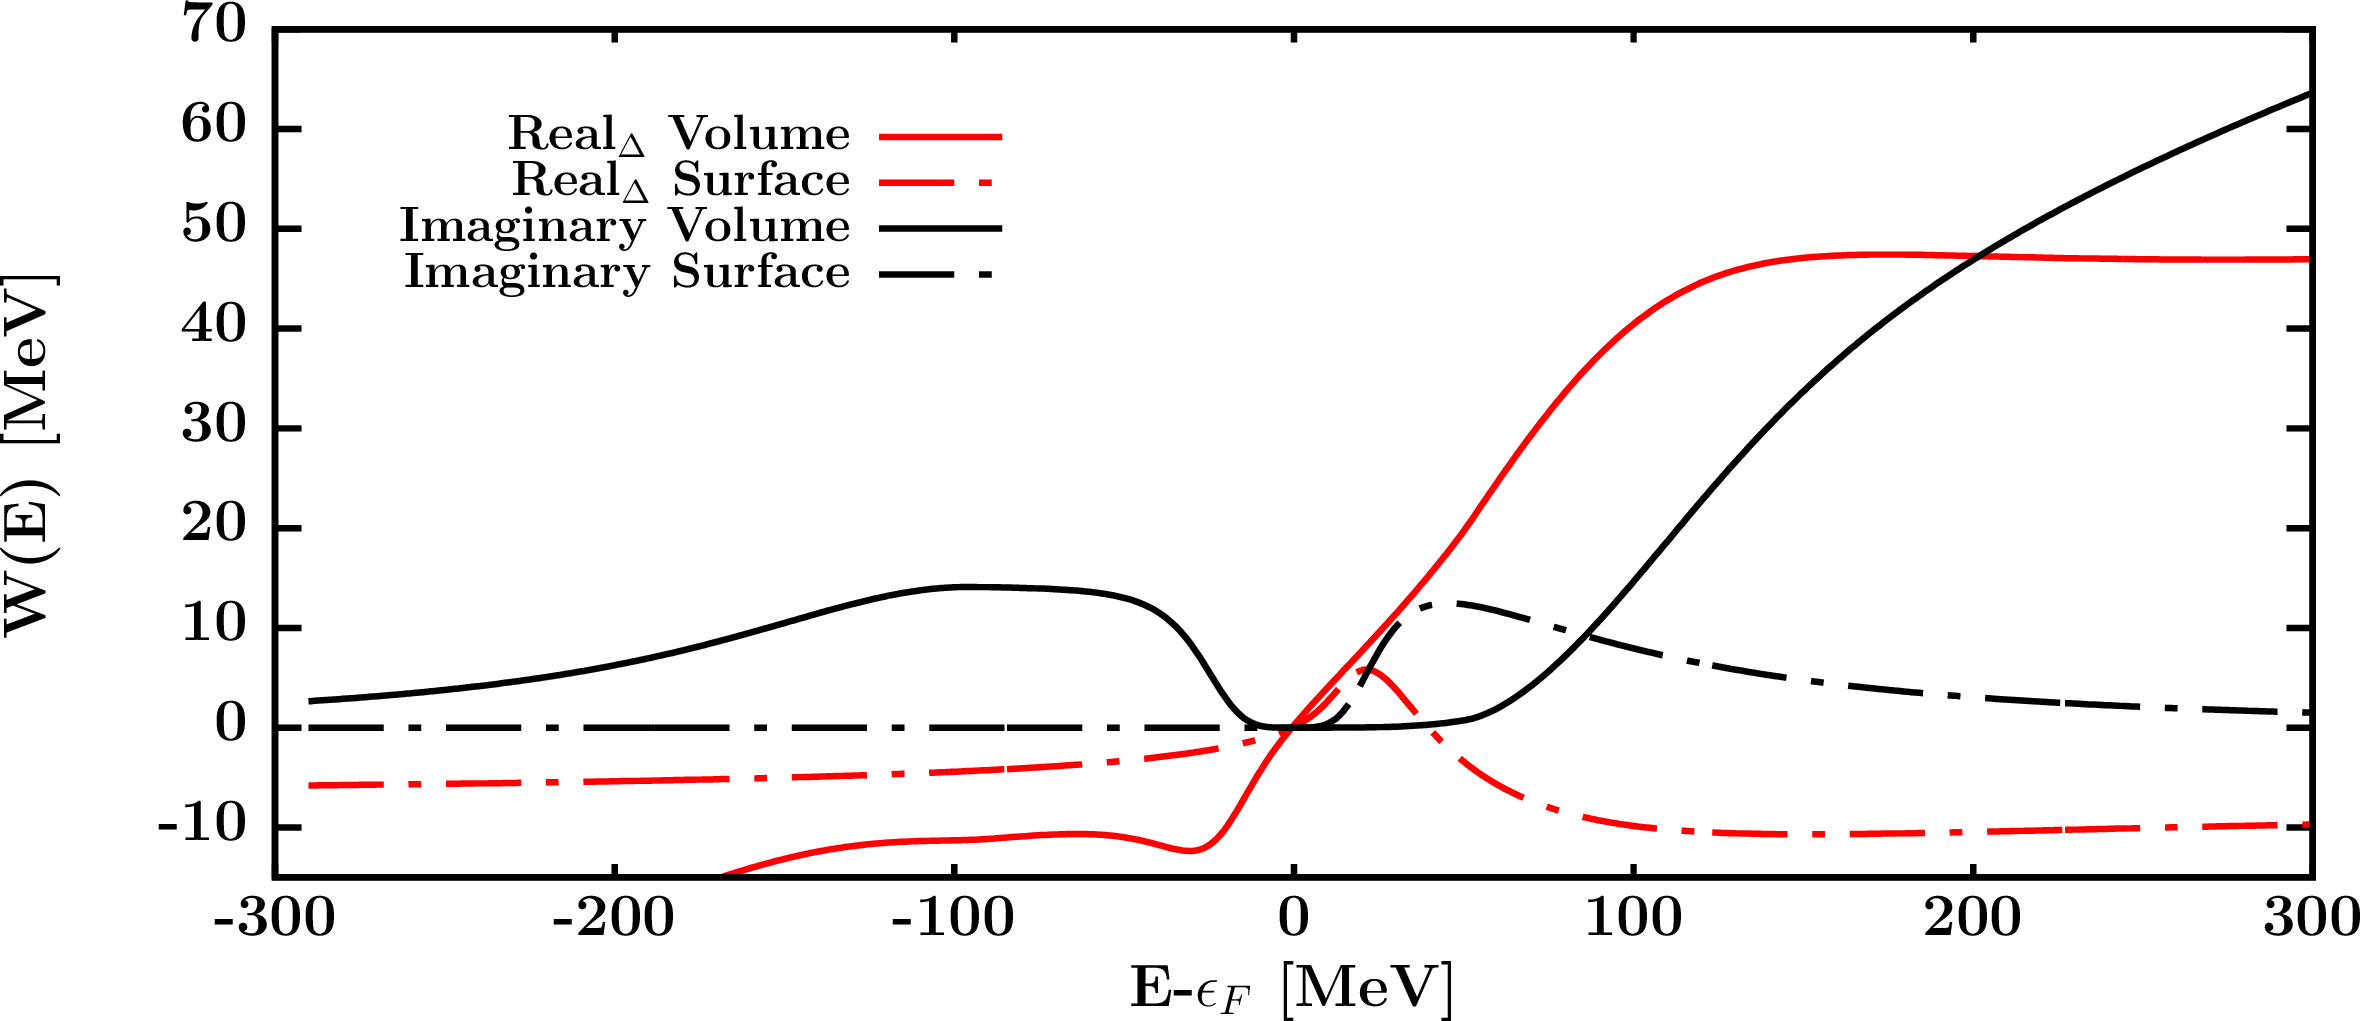
\includegraphics[width = 0.9\textwidth]{figures/o16_neutronPotentials.png}
\caption{Visualization of DOM optical potential components for neutrons on
$^{16}O$}
\label{o16NeutronPotentials}
\end{center}
\end{figure}

\begin{figure}
\begin{center}
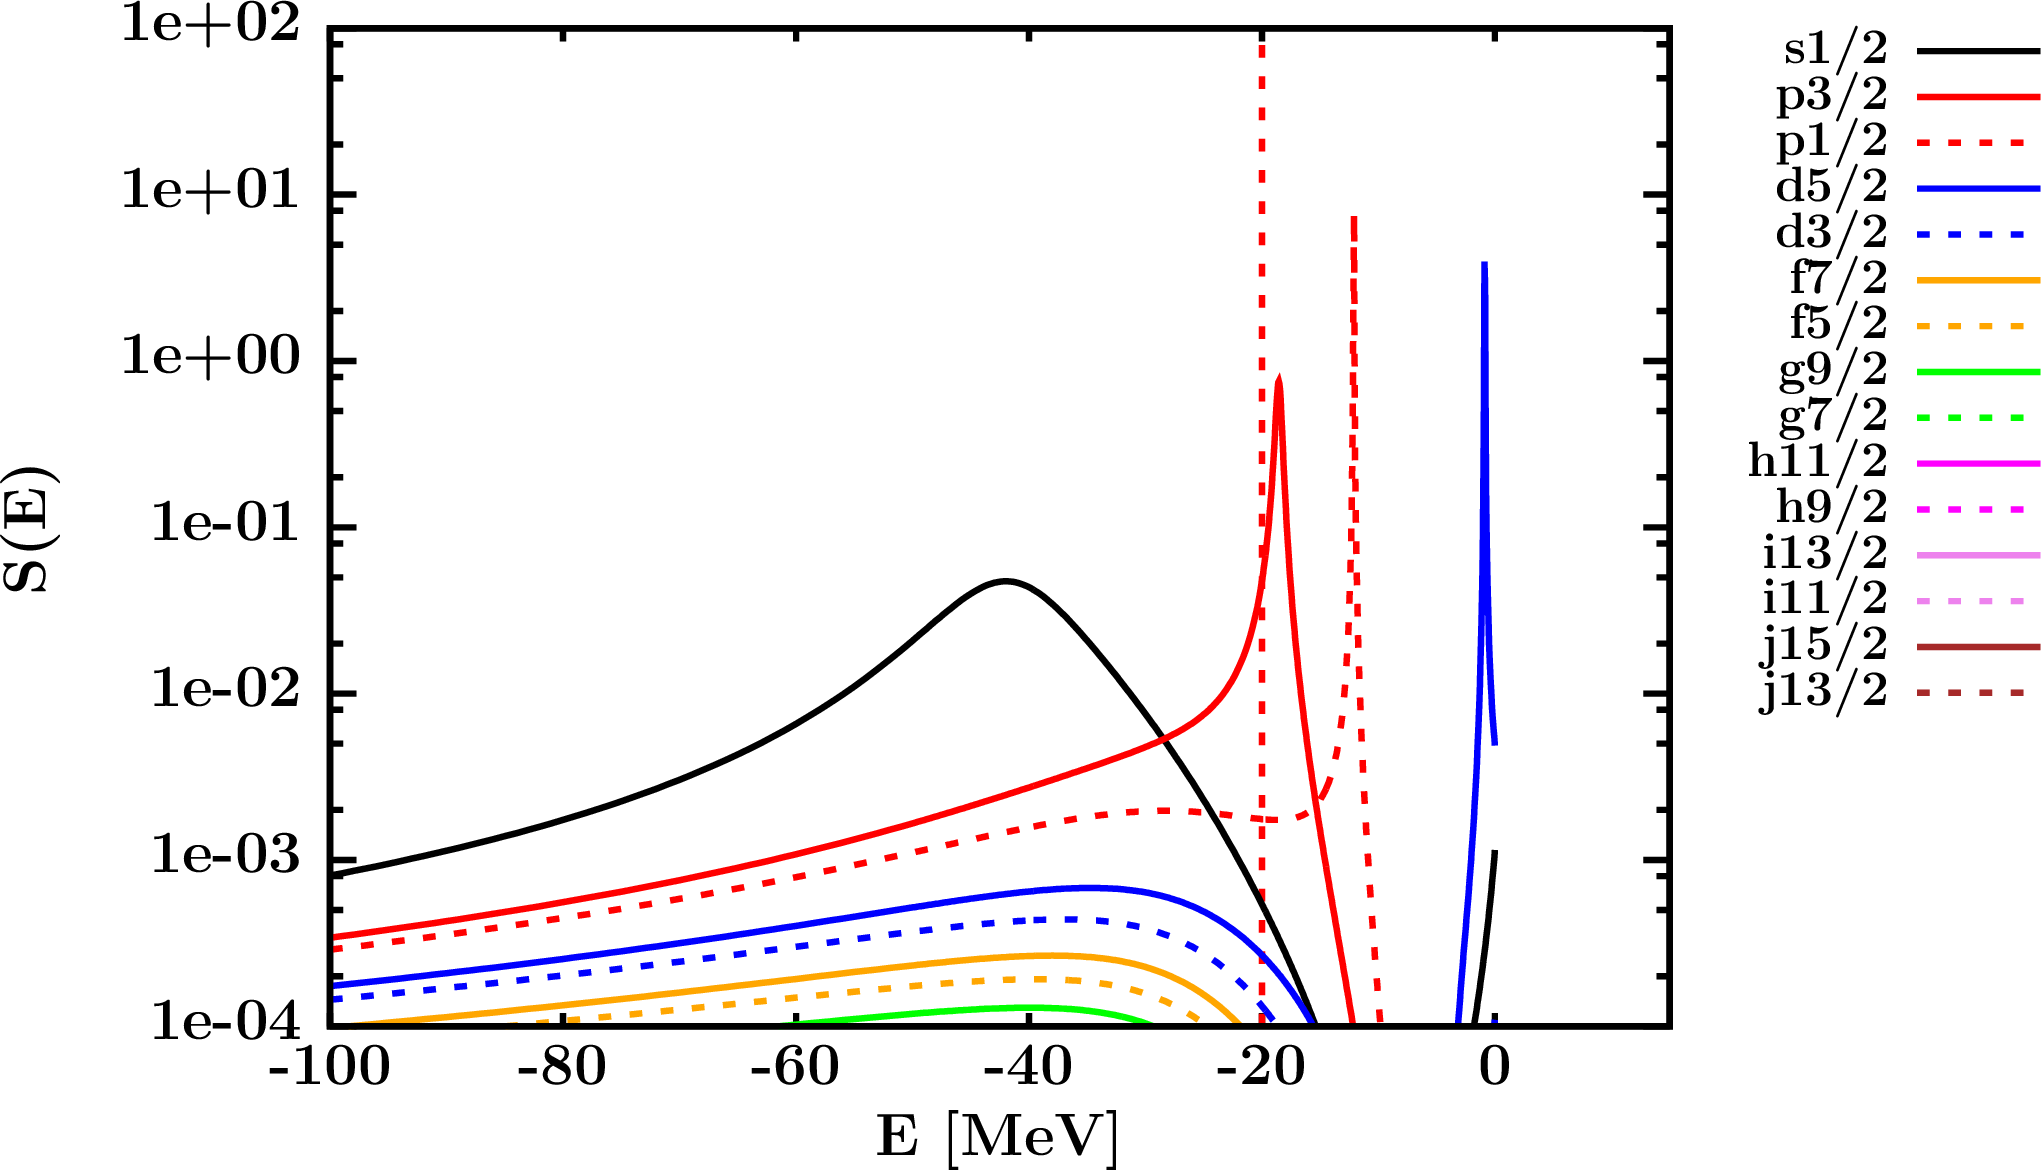
\includegraphics[width = 0.9\textwidth]{figures/o16_protonSpectralFunctions.png}
\caption{DOM calculation of $^{16}O$ proton spectral functions}
\label{o16ProtonSpectralFunctions}
\end{center}
\end{figure}


\begin{figure}
\begin{center}
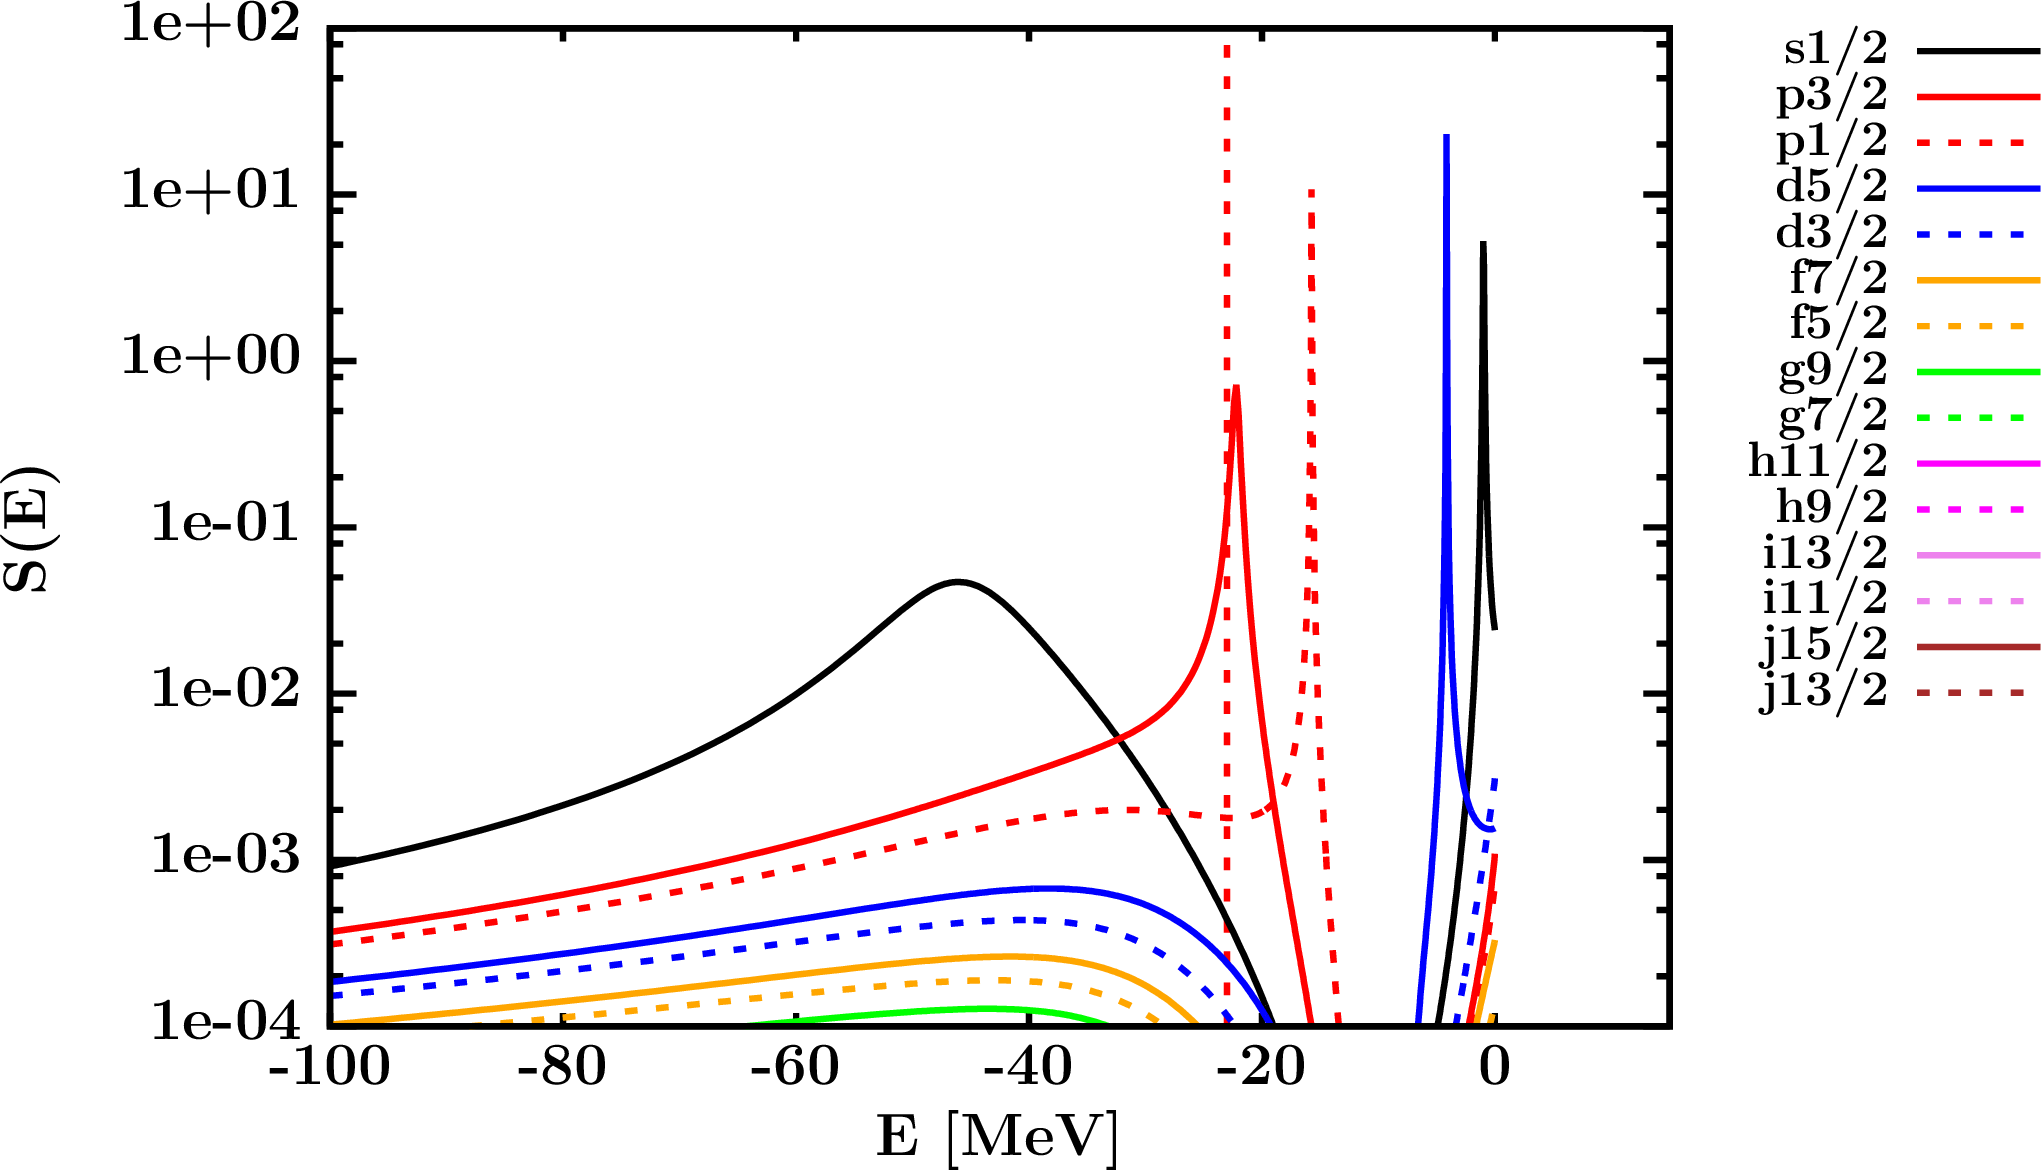
\includegraphics[width = 0.9\textwidth]{figures/o16_neutronSpectralFunctions.png}
\caption{DOM calculation of $^{16}O$ neutron spectral functions}
\label{o16NeutronSpectralFunctions}
\end{center}
\end{figure}

\begin{figure}
\begin{center}
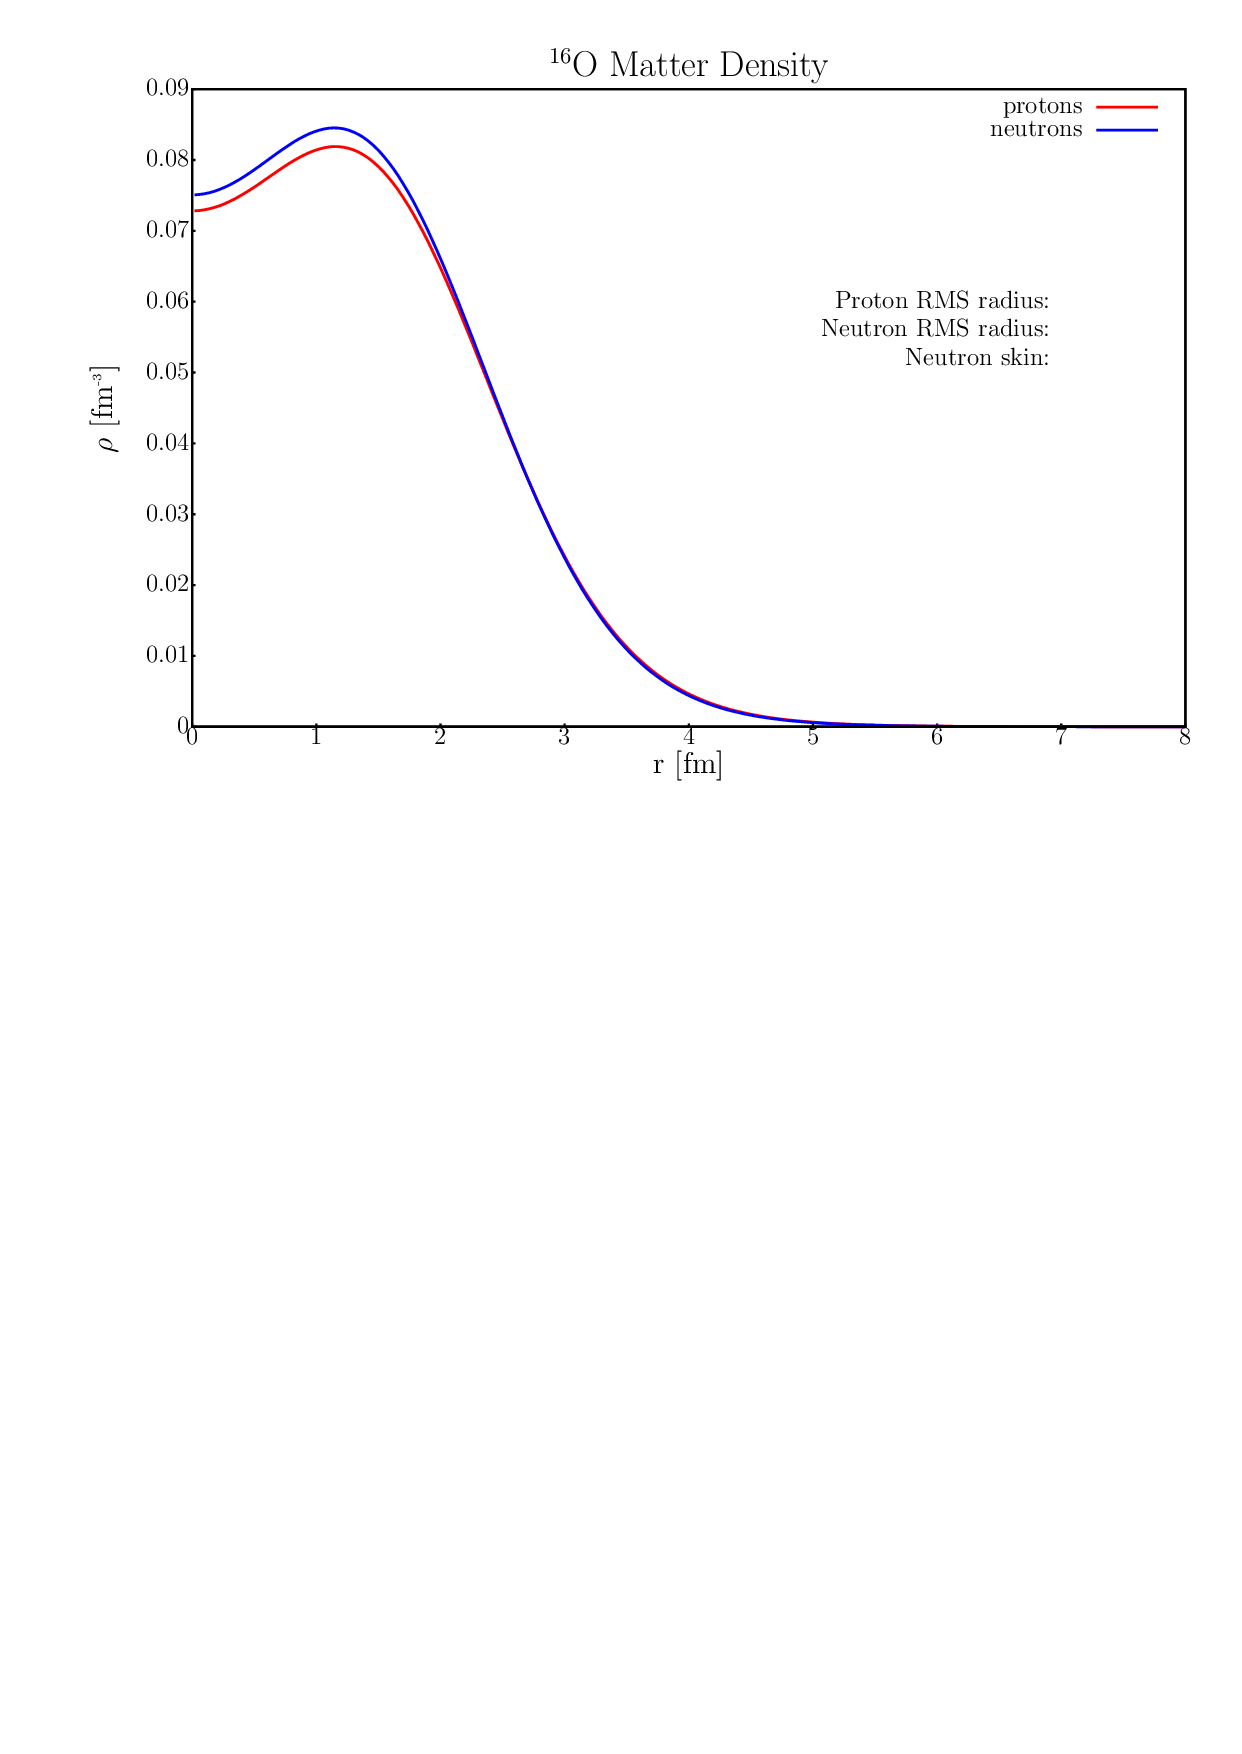
\includegraphics[width = 0.9\textwidth]{figures/o16_matterDensity.png}
\caption{DOM prediction of $^{16}O$ matter density}
\label{o16MatterDensity}
\end{center}
\end{figure}

%\begin{table}
%  \begin{center}
%    \caption{Calibration beams and the energies generated with the degraders.}\label{CBeams}
%  \begin{tabular}{ccccc}
%    \hline \hline
%    Species & Energy & Target & Thickness & Degraded Energy  \\ 
%            & [MeV/A] & &[mg/cm$^2$] & [MeV/A] \\
%     \hline
%    $p$ & 24.2 &  Au & 20.0 & 24.0   \\
%           &  & Al & 429 & 15.8 \\
%    \hline
%    $d$ & 24.2 &  Au &20.0 & 24.1 \\
%            & & Al & 429 &20.3 \\
%    & &  Al & 858 & 15.8 \\
%            & 12.0 &  Au & 20.0 & 11.9 \\
%    \hline
%    $\alpha$ & 24.0 &  Au & 20.0 & 23.8 \\
%     & & Al & 429 &15.6 \\
%    \hline \hline
%  \end{tabular}
%\end{center}
%\end{table}

\subsection{Trends across all fitted nuclei}

\afterpage{\clearpage}
